\documentclass[a4paper,12pt,oneside,final]{article}
\usepackage[pdftex]{graphicx}
\usepackage[T1]{fontenc}
\usepackage{titlesec, color}
\usepackage{anysize}
\usepackage{listings}
\usepackage{subfigure} 

\usepackage[latin1]{inputenc}
\usepackage{graphicx}
\usepackage{amssymb}
\usepackage{epstopdf}
\usepackage{color}
\lstset{
language=JAVA,
basicstyle=\footnotesize, 
keywordstyle=\color{keywordcolor}\bfseries, %\underbar
backgroundcolor=\color{white}, 
identifierstyle=, 
commentstyle=\color{blue} \textit, 
stringstyle=\ttfamily, 
showstringspaces=false,
captionpos=b,
frame=trBL,
}
\definecolor{keywordcolor}{rgb}{0.8,0.1,0.5}

\newenvironment{changemargin}[2]{\begin{list}{}{%
\setlength{\topsep}{0pt}%
\setlength{\leftmargin}{0pt}%
\setlength{\rightmargin}{0pt}%
\setlength{\listparindent}{\parindent}%
\setlength{\itemindent}{\parindent}%
\setlength{\parsep}{0pt plus 1pt}%
\addtolength{\leftmargin}{#1}%
\addtolength{\rightmargin}{#2}%
}\item }{\end{list}}
\marginsize{30mm}{30mm}{20mm}{20mm}
\definecolor{gray75}{gray}{0.75}
\newcommand{\hsp}{\hspace{20pt}}
\author{
    Yufei Wang (yw6312, s5) \\ 
    Paul Gribelyuk (pg1312, a5) \\
    Yawei Li (yl8012, s5) \\ 
    Jun He (jh1212, s5) \\
    Xiaoxing Yang (xy212, s5)
}
\makeatother

\title{\Huge Software Engineering for Industry \\ Coursework 2: AcmeTelecom Billing System}

\begin{document}
\maketitle

\newpage

\section{Introduction} % paul
\paragraph{}
This report covers the analysis, testing, refactoring, and re-engineering of the AcmeTelecom billing system.  We saw our responsibility as two-fold: to build a well-tested, easy to maintain, coherent piece of software, and to use that software to implement a billing algorithm which fairly bills clients according to the time they spent calling during peak and off-peak times.  We relied heavily on Test Driven Development (TDD) practices in the way we devised tests, using unit tests to assert the state of our system, and mock tests to verify its behaviour.  To put in place tests for the initial code base, we were forced to make decisions about design patterns present (such as the singleton pattern in \verb+HtmlPrinter+) as well as make heavy use of interfaces to allow the JMock libraries to interact with out code.  Once satisfied with the initial functionality, we wrote integration tests and opened the development process to the business expert by writing a DSL around the components most responsible for how the billing system determines rates for customers.

\paragraph{}
We used these specificaitons to guide us in the design phase, where we ultimately chose to preserve the structure of the \verb+BillingSystem+ object as the class which is the central component collecting call information and passing them on to the \verb+BillGenerator+ rather than deciding what those calls shoudl cost.  We externalized that business logic by putting it in a separate class, thus making the original class more cohesive and simplifying the process to incorporate future changes.  We used a modern version control system (\emph{git}) and a continous integration server to manage the testing framework and automatically build after each commit.  Dependency matrix analysis helped to gain a big-picture understanding of the codebase without reading every line.

\paragraph{}
We were also careful not to over-optimize and decided to keep the general design of the system in tact, since it also inter-operates with other external libraries throughout the AcmeTelecom organization.  If we were to implement a brand new design, we would have loosened the coupling further by using Dependency Inversion model wherever possible and definining how interfaces should communicate rather than how concrete classes should change state.
	

\section{Analysis of Original Code} % paul
\paragraph{}
The original code for the Billing System was well structured, though lacking any tests, so a look at the dependency structure was needed to begin to analyze where work would need to be done.  We have included a diagram of this here:
\begin{figure}[!h]
\begin{changemargin}{-20mm}{-20mm}
\center
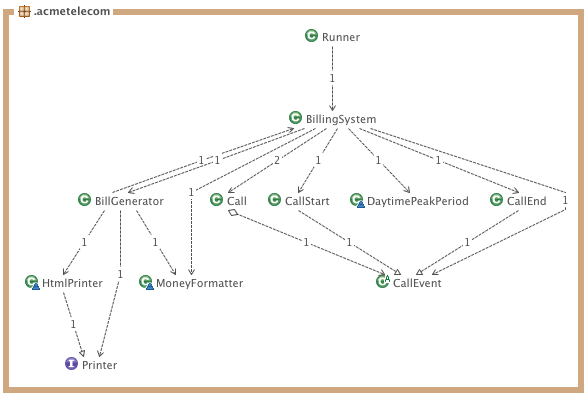
\includegraphics[scale=0.55]{Original_Structure.png}
\caption{Original Dependency Structure of the Billing System}
\end{changemargin}
\end{figure}
The 3-layer architecture is preferable in this case, since it is an in-house system with a small well-defined userbase and more a intricate architecture pattern would not be needed. The code also lacks interfaces to begin to easily write tests, especially with JMock, which requires an interface to mock behaviour.  

\paragraph{}
The \verb+CallEvent+ is the basic building block of a \verb+Call+, which consists of a \verb+CallStart+ and a \verb+CallEnd+, which both inherit from \verb+CallEvent+.  The \verb+BillingSystem+ receives method calls to \verb+callInitiated+ and \verb+callCompleted+ and logs them to a \verb+List<>+ object.  A call to the \verb+createCustomerBills+ calculates the costs of each call as it occurs in teh list, and then dispatches this list of \verb+Calls+ to the \verb+BillGenerator+ by invoking \verb+send+.  The \verb+BillGenerator+ uses an \verb+HtmlPrinter+ to output the results into HTML (in this example, to \verb+System.out+).  Other classes, such as \verb+MoneyFormatter+ and \verb+DaytimePeakPeriod+ act as helper classes.

\section{Refactoring and Testing} % fred (maybe and paul)
Creating interfaces for testing purposes
Creating Mock tests
Creating Unit tests for container classes
Breaking \verb+HtmlPrinter+ singleton interface and changing constructor to take a different \verb+PrintStream+ other than \verb+System.out+.

Extracted calculation part of original \verb+BillingSystem+ into a new class to allow flexibility in future design.

\section{Creating a DSL} % fred

\section{Implementing the New Billing System}  % juno
% here we talk about the way to design new system and how the calculations happen
% include some important lines of code as examples
\paragraph{}
As mentioned in the "Refactoring and Testing" section, we extracted the fee calculation part out of the the \verb+BillingSystem+ class. A new package \verb+rate+ was created under \verb+com.acmetelecom+, dealing with specific cost calculation. An interface \verb+RateEngine+ was provided to communicate with other parts of the system. 
\begin{lstlisting}[ ]
     public interface RateEngine {
   	 public Cost calculateCost(Call call, Tariff tariff);
     }
\end{lstlisting}
The interface only contains one public method which requires a \verb+Call+ and the \verb+Tariff+ for that call and returns the \verb+Cost+.  There are several advantages of extracting the cost calculation into a seperate package. Firstly, we decoupled the original system, making it more reusable. Additionally, the whole system is more flexible to be implemented with different rate calculation in the future because different implementations are possible for one interface. This feature immediately helped us when implementing the new billing system. The concrete implementation of the original cost calculation logic was built into the \verb+ProfitableRateEngine+ class, which will compute cost under the peak rate as long as the call duration is touching peak. In order to calculate the cost fair to customers, alternatively, we created a new implementation of \verb+RateEngine+, called \verb+PeakSeperateOffPeakRateEngine+ to tackle the new cost calculation standard. The switching cost of the original billing system then is very low as we can easily achieve new features by changing \verb+RateEngine+ instance initialization from \verb+ProfitableRateEngine+ to \verb+PeakSeperateOffPeakRateEngine+ without breaking any other codes.

\paragraph{}
All new cost calculation logics were handled within the new rate engine implementation. The general idea is that we introduced two variables \verb+peakTime+ and \verb+offPeakTime+. For different call lasting situations, in order to get cost, we multiply the \verb+peakTime+ and \verb+offPeakTime+ to different rates. The difficult point for this idea is that, we had to analyze the call duration such that we can accurately seperate  the peak time and off peak time. For making the class tidy and readable, a helper function \verb+calculateDuration(Call call)+ was added to analyze the call duration. Since we relied on the TDD development process, we've prepared all possible call senarios (mentioned later).It is convinient to program the duration logic based on the senarios. There are basically two situations; a call finished in one day and a call lasted overnight. For each situation, different conditions could be applied around the peak start point and peak end point. In the algorithm, we make use of the \verb+Calender+ API, helping us retrieve the Hour, Miniute, and Second from a \verb+Date+ type.  By comparing the call start point and call end point to those critical peak points, we differentiate various situations and figure out the peak time and off peak time.

% \emph{emphasize} \textbf{boldface}

\section{Acceptance Tests} % cici and juno
\paragraph{}
We adopted the Framework for Integrated Tesing (FIT) to exam our end-to-end test. In FIT html requirement documents, we wrote 9 different cases according to different factors, i.e. starting point, ending point, and duration (As shown below). This covered all possible situations a customer may come across.
\begin{figure}[!h]
\begin{changemargin}{-20mm}{-20mm}
\center
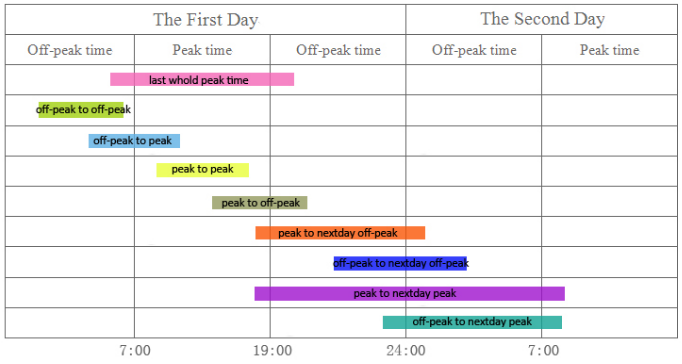
\includegraphics[scale=0.70]{fit-cases.png}
\caption{Acceptance-Test Scenario (assuming 7:00-19:00 peak period)}
\end{changemargin}
\end{figure}

In the requirement documents, by default, the system is initialized as peak time starts at 7:00:00 and ends at 19:00:00. A customer information table will be given to represent all customers that are eligible to have a bill. Different calls are speicified in the Call table, which simulates the call process. The last table is showing the bills and this is the table that will be examed by the test. In order to execute FIT test, we wrote some classes to parse these tables. 
\begin{center}
    \begin{tabular}{ | l | p{8cm} |}
    \hline
    Class Name: &  Description: \\  \hline
    SystemUnderTest  & Create instances for testing \\  \hline
    GivenTheSystemIsInitialized & Reset the test system \\  \hline
    GivenPeakPeriod  & Set the peak time period \\  \hline
    GivenTheFollowingCustomer: & Store customer information into FakeCustomerDatabase\\  \hline
    GivenTheseCallsAreMade: & Record calls into billing system \\  \hline
   TheBillShows: & Generate customer bills for comparision \\
   \hline
    \end{tabular}
\end{center}

\paragraph{}
It is worth noting that we added three fake classes  \verb+FakeCustomerDatabase+, \verb+FakeGenerator+, \verb+FakePrinter+, to facilitate our FIT test. This is because CentralCustomerDatabase is a singleton from other system and we do not have access to that database. While there is a CustomerDatabase interface, we can have our own fake database implementation based on ArrayList to save customers information from FIT requirements. FakeGenerator and FakePrinter are created to fullfil the table output format in the requirement. 

\begin{figure}
\centering
\mbox{\subfigure{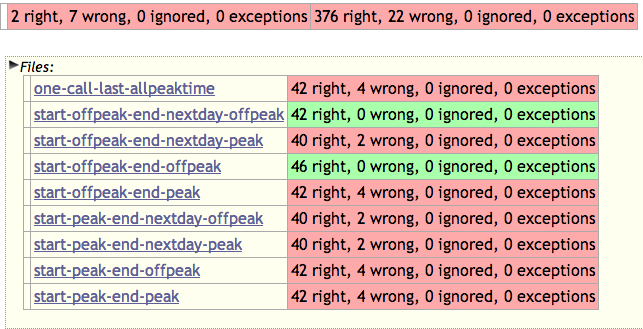
\includegraphics[width=3in]{FIT-result-before-change.png}
\quad
\subfigure{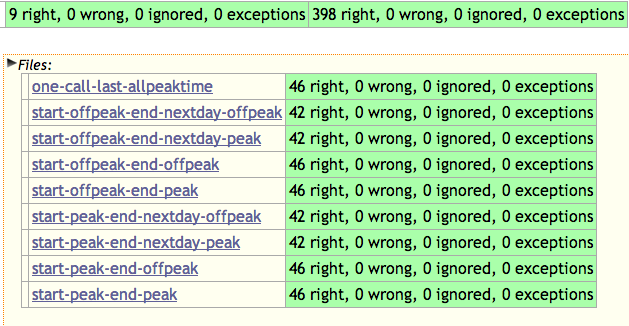
\includegraphics[width=3in]{FIT-result-after-change.png} }}}
\caption{FIT Results Comparision}
\end{figure}

When running the FIT scenarios running with the original rate calculation engine, we failed in most FIT test because the actual costs were not produced as expections. After refactoring with the usage of the new RateEngine implementation, we made all tests pass, which means we met the need of  specification. 



% \begin{figure}[!h]
% \begin{changemargin}{-20mm}{-20mm}
% \center
% \includegraphics[scale=1]{file_name.jpg}
% \caption{Caption string}
% \end{changemargin}
% \end{figure}i

\section{Conclusions and Recommendations} % leah
\paragraph{}
Tools used (Git, Jenkins, IntelliJ Coverage Report, IntelliJ Dependency Matrix).  Problems enountered like refactoring for Tiny Types, Mocking with concreted classes rather than interfaces.
% \blindtext
\end{document}
